\chapter{An Implementational Framework for the PEM} \label{ch:implementation}
%
The implementation of a given partitioned element method must address two primary challenges: the subdivision of an element into cells, and the solution of shape function boundary value problems by way of the chosen PEM formulation. The first of these two tasks may be accomplished in various ways, some of them more complicated than others. Herein we propose a relatively simple element partitioning algorithm which necessitates that the elements and their faces be simply connected, and star-convex.

The present framework is directed at obtaining DG-FEM approximations to harmonic shape functions on arbitrary polyhera -- i.e. solving (\ref{eq:dg_poisson}) on an appropriately defined partition of the element.

\section{Arbitrary Polytopal Meshes}



\subsection{Polytopal Mesh Data Structures}

	There are multiple ways in which the geometry of a given polyhedral element $\Omega$ may be represented within a finite element code. Ideally, however, the chosen data structure should be made as compact as possible, for the purposes of minimizing the storage requirements of a single element. This section describes a few basic data structures for storing arbitrary polgonal and polyhedral shapes within an unstructured finite element mesh.
	
	It is assumed that the mesh geometry for the finite element discretiztion of the model problem described in chapter \ref{ch:solid_mechanics} may be generically characterized by:
	\begin{itemize}
		\item A list of all nodal coordinates $\left\{ \mathbf{X}_a \right\}_{a=1}^{N_V}$. The sub-index $a \in 1, \ldots, N_V$ induces a \textit{global node ID} ascribed to each node.
		\item A list of all elements $\left\{ \Omega_{e} \right\}_{e = 1}^{N_e}$ where $\Omega_{e} \subset \mathcal{B}_0$.
		\item A list of all faces $\left\{ F_{b} \right\}_{e = 1}^{N_F}$ where $F_{b} \subset \Gamma^N_0$ to which traction boundary conditions are assigned.
	\end{itemize}
	
	In a simple finite element mesh consisting of arbitrary polyhedral elements, it is suggested that each polyhedral element $\Omega_e$ be represented by the following sets of data:
	\begin{itemize}
		\item A list of the global node IDs $\left\{ a_i \right\}_{i=1}^{N^e_V}$ which belong to $\Omega_e$. The sub-index $i \in 1, \ldots, N^e_V$ induces a \textit{local node ID} for each node, particular to the element $\Omega_e$.
		\item A list of the polygonal faces $\left\{ F_{c} \right\}_{c=1}^{N^e_F}$ which belong to $\partial \Omega_e$; each polygonal face $F_c$ is in turn represented by a cycle of local node IDs $\left\{ n_i \right\}_{i=1}^{N^c_V}$, which further determine each face's outward orientation with respect to the element $\Omega_e$.
	\end{itemize}
	An illustration of this organization for a given polyhedron $\Omega_e$ is provided in Figure \ref{fig:fig:polyhedron_data}.
	\begin{figure} [!ht]
		\centering
		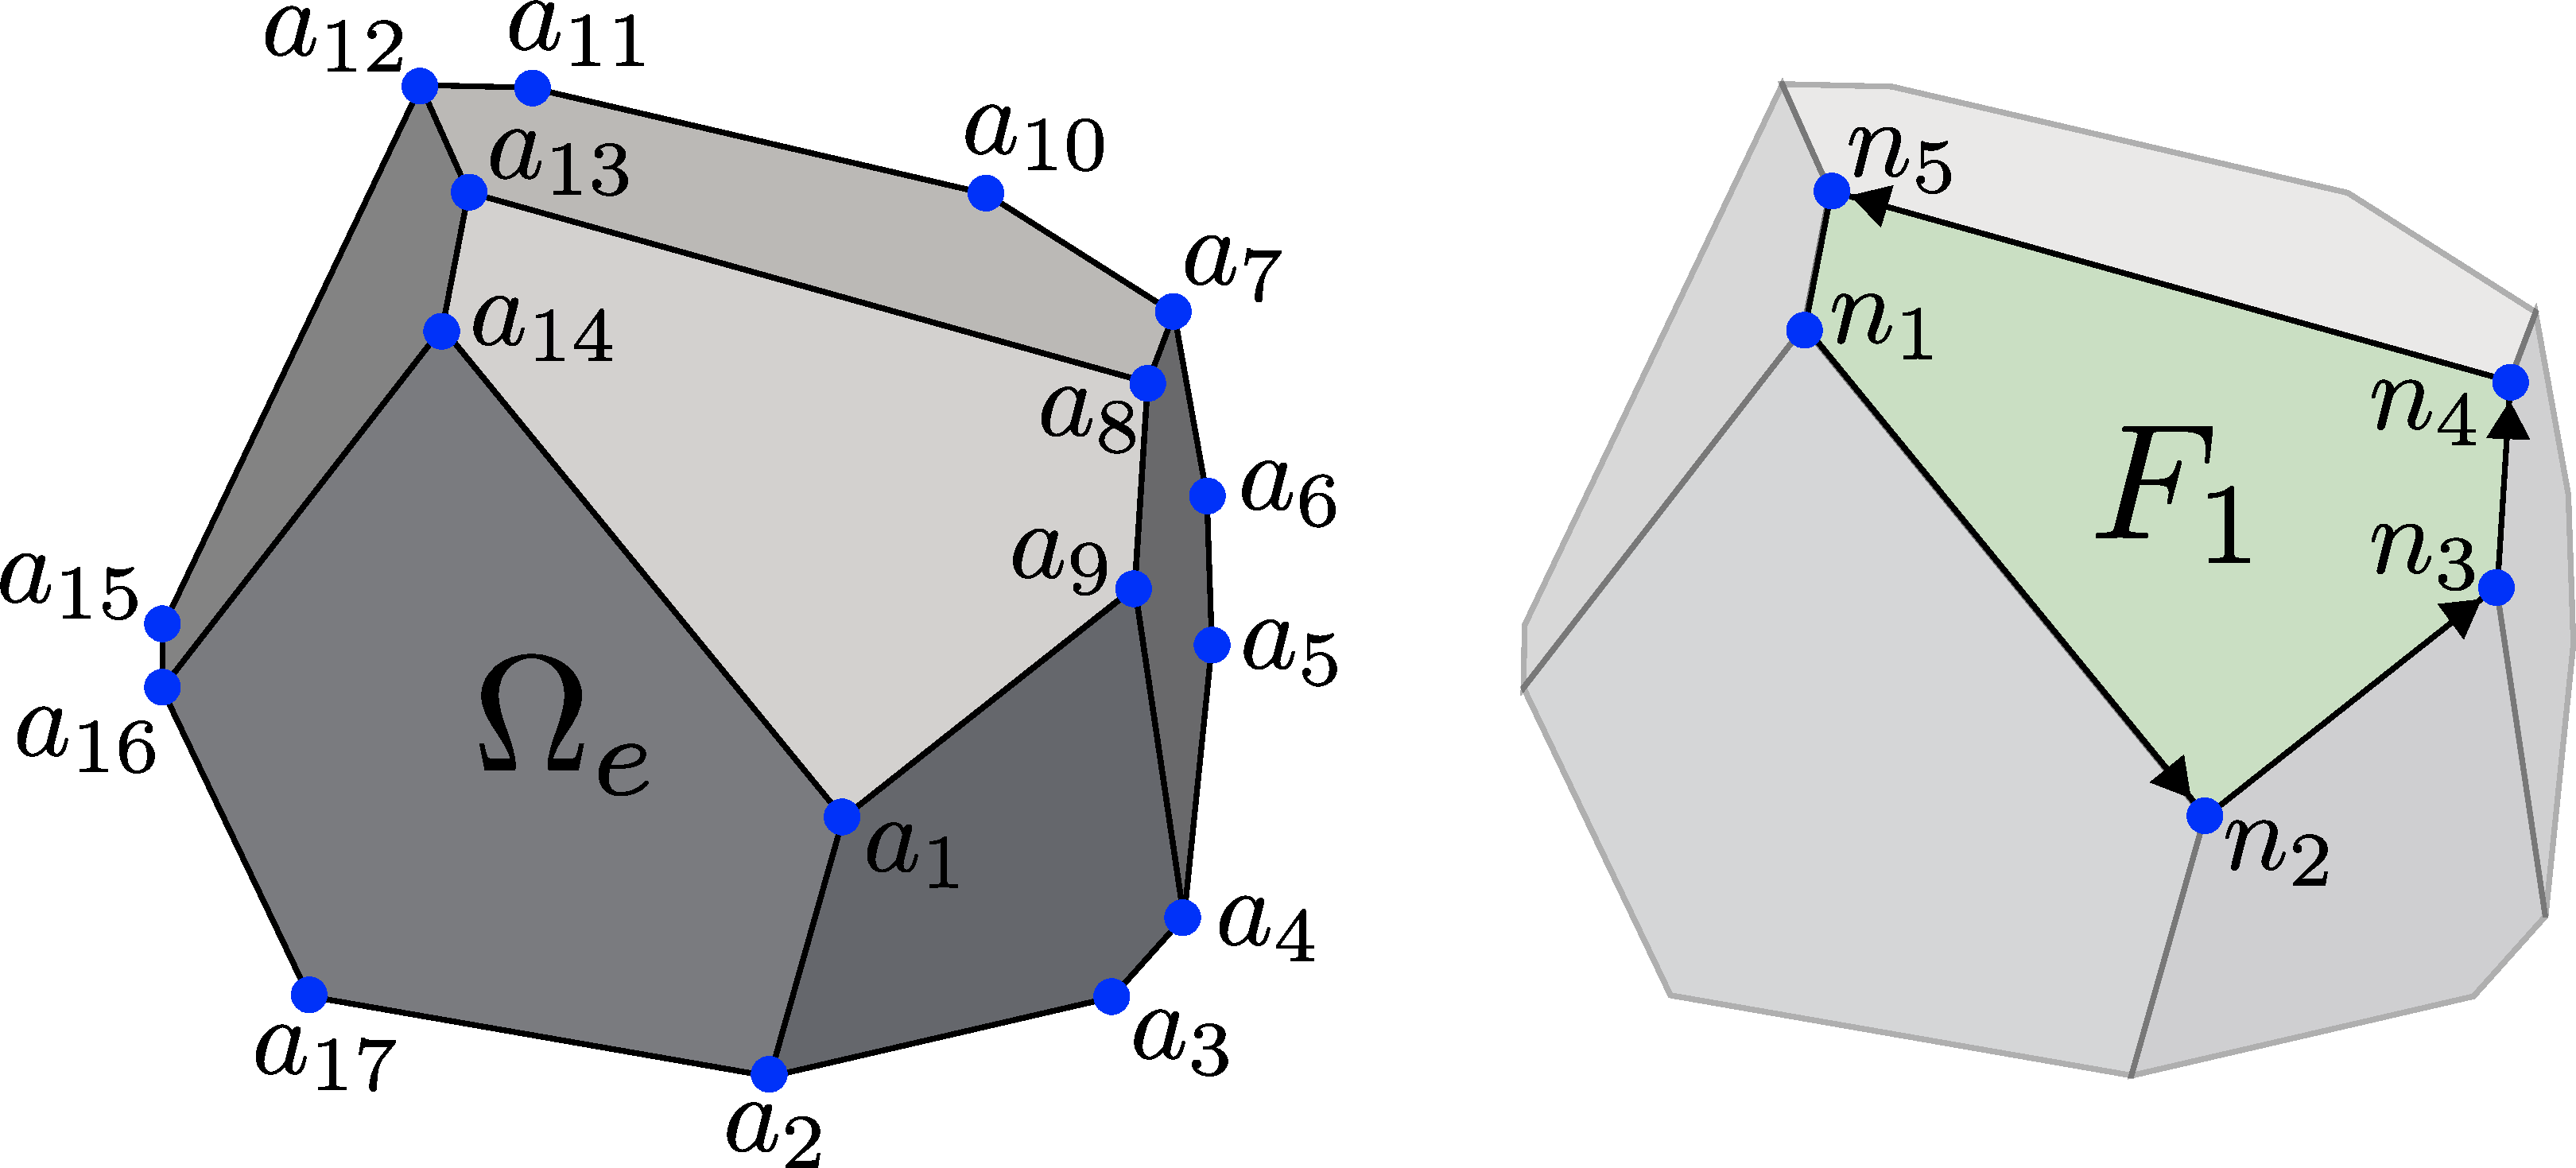
\includegraphics[width = 6.0in]{figures/polyhedron_data.pdf}
		\caption{Illustration of the data used to describe an arbitrary polyhedron $\Omega_e$. The local node ID ordering for the face $F_1$ shown would be $\left\{ n_i \right\}_{i=1}^{N^c_V} = \left\{ 14, \, 1, \, 9, \, 8, \, 13 \right\}$.}
		\label{fig:polyhedron_data}
	\end{figure}
	
	A given polygonal face $F_b \subset \Gamma^N_0$ will similarly be represented by:
	\begin{itemize}
		\item A list of the global node IDs $\left\{ a_i \right\}_{i=1}^{N^b_V}$ which belong to $F_b$.
		\item A list of the linear edges $\left\{ E_{c} \right\}_{c=1}^{N^b_E}$ which belong to $\partial F_b$; each linear edge $E_c$ is in turn represented as an ordered list of local node IDs $\left\{ n_i \right\}_{i=1}^{N^c_V}$.
	\end{itemize}
	
\section{Element Partitioning Schemes}

\subsection{Edge-Based Partitioning for Star-Convex Elements}

	A star-convex shape $\Omega$ is one for which there exists some point $\mathbf{X}^{\Omega}_0 \in \Omega$ such that the line segment connecting any point $\mathbf{X} \in \Omega$ to $\mathbf{X}^{\Omega}_0$ is wholly contained within $\Omega$. For a polyhedral element $\Omega$ which is star-convex, this further implies that each polygonal face $F \subset \partial \Omega$ is also star-convex with respect to a point $\mathbf{X}^{F}_0 \in F$. Any linear edge $E \subset \partial F$ is of course star-convex with respect to any point $\mathbf{X} \in E$. Such a figure $\Omega$ may be decomposed into tetrahedra in a straightforward manner. Moreover, each face $F \subset \partial \Omega$ can be decomposed into triangles by a similar process.
	
	A simple and efficient partitioning scheme is described for elements $\Omega_e$ (and faces $F_b$) which are star-convex with respect to their vertex-averaged centroid $\bar{\mathbf{X}}^{\Omega_e}_0$ (or $\bar{\mathbf{X}}^{F_b}_0$), i.e.
	\begin{equation}
		\bar{\mathbf{X}}^{\Omega_e}_0 = \frac{1}{N^e_V} \sum_{i = 1}^{N^e_V} \mathbf{X}_{a_i}, \quad \text{and} \quad \bar{\mathbf{X}}^{F_b}_0 = \frac{1}{N^b_V} \sum_{i = 1}^{N^b_V} \mathbf{X}_{a_i}.
	\end{equation}
	
	For a given polyhedral element $\Omega_e$, the algorithm proceeds in several steps:
	\begin{itemize}
		\item[1.)] Identify all edges of the polyhedron, and subdivide them into linear segements; each segment should adjoin two consecutive nodes of a given edge.
		\item[2.)] For each face, compute its vertex-averaged centroid $\bar{\mathbf{X}}^{F_c}_0$, and subdivide the face into triangular facets which emanate from $\bar{\mathbf{X}}^{F_c}_0$; each facet should share at most two segments (at least one segment) with $\partial F_c$.
		\item[3a.)] Compute the element's vertex-averaged centroid $\bar{\mathbf{X}}^{\Omega_e}_0$, and subdivide the element into tetrahedra which emanate from $\bar{\mathbf{X}}^{\Omega_e}_0$; each tetrahedron should share a single facet with $\partial \Omega_e$.
		\item[3b.)] Lump into cells any tetrahedra which share a segment belonging to an edge of $\Omega_e$; each cell should consist of exactly two tetrahedra.
	\end{itemize}
	A similar agorithm may be applied to each face $F_b$, entailing only the first two steps. An illustration of this process is depicted in Figure \ref{fig:partitioning_algorithm}.
	\begin{figure} [!ht]
		\centering
		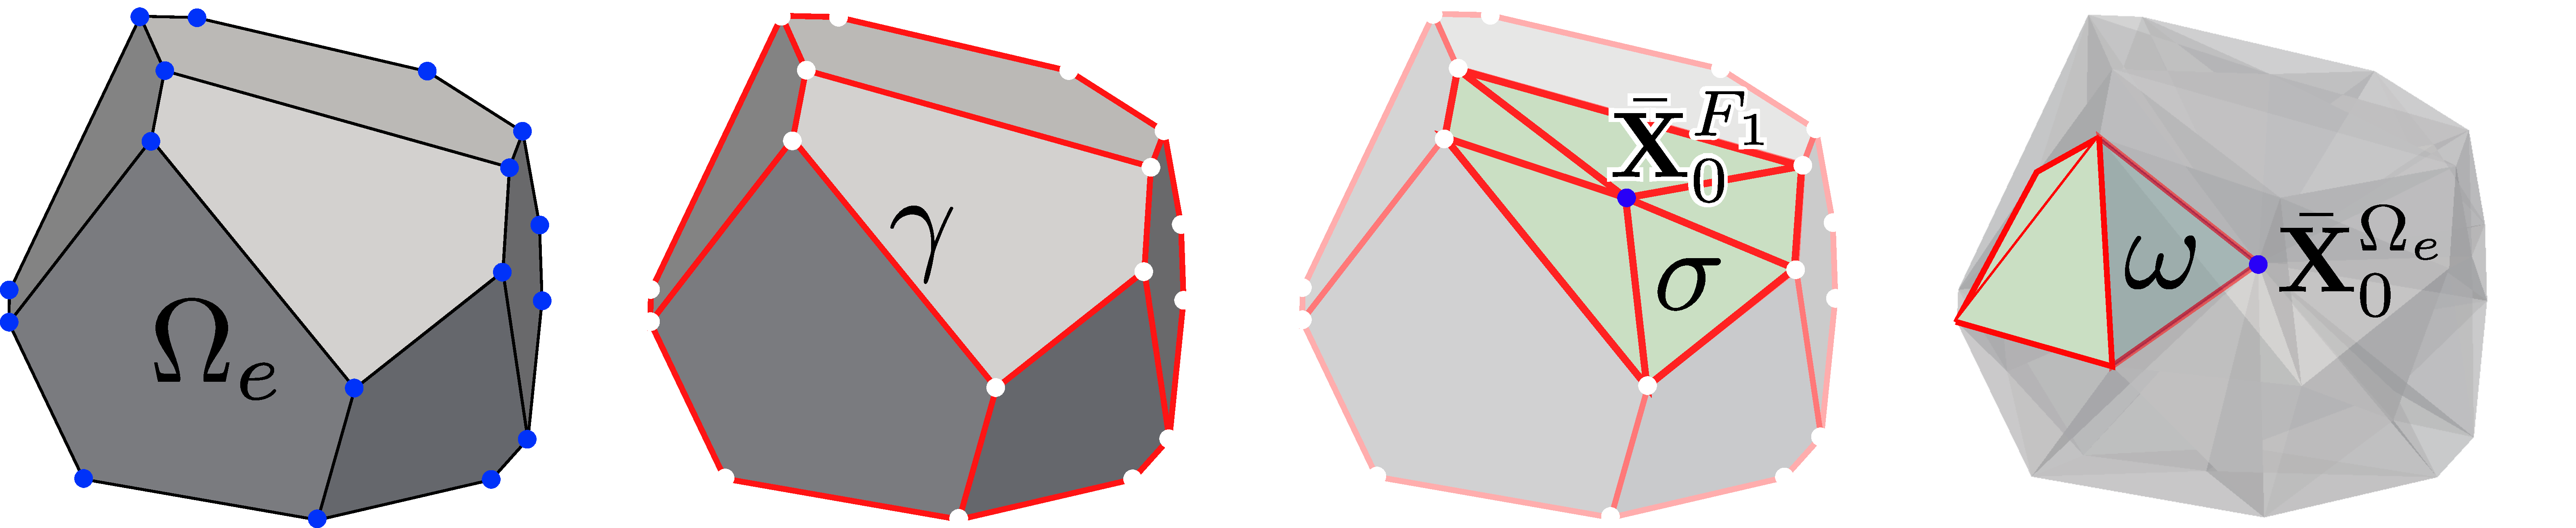
\includegraphics[width = 6.0in]{figures/partitioning_algorithm.pdf}
		\caption{The resulting segment, facet, and cell decomposition for the proposed edge-based partitioning algorithm.}
		\label{fig:partitioning_algorithm}
	\end{figure}
	

\section{Abstract Data Structures and Generic Programming Concepts}

	Because the PEM consists of solving a set of 1D, 2D, and 3D problems on each edge, face, and element, there arise a number of apparent similarities between these problems of variable dimension. Namely, the geometric data describing each cell, facet, segment and vertex may be abstracted through the use of generic parent-child (tree-based) data structures. Instead of requiring a separate implementation for the solution of each 1D, 2D, 3D problem, the use of generic programming paradigms are exploited to facilitate a single, unified implementation which is agnostic to the dimensionality of the problem being solved.
	
\subsection*{Geometric Entities}

	\textit{Entities} are the atomic units of the element's geometric partition. Entities include: polyhedral cells, polygonal facets, linear segments, and verticies. A $d-$dimensional entity is uniquely defined by its $(d-1)$-dimensional faces (children), and their corresponding outward orientations (normal directions). These faces are in turn $(d-1)$-dimensional entities, defined in terms of their $(d-2)$-dimensional children. An entity of dimension $0$ (a vertex) is identified as having no children.
	
	Consequently, each geometric entity may be viewed as a node in a corresponding tree data structure, as illustrated in Figure \ref{fig:entity_tree}, where the height of a given entity within the tree indicates its dimensionality.
	\begin{figure} [!ht]
		\centering
		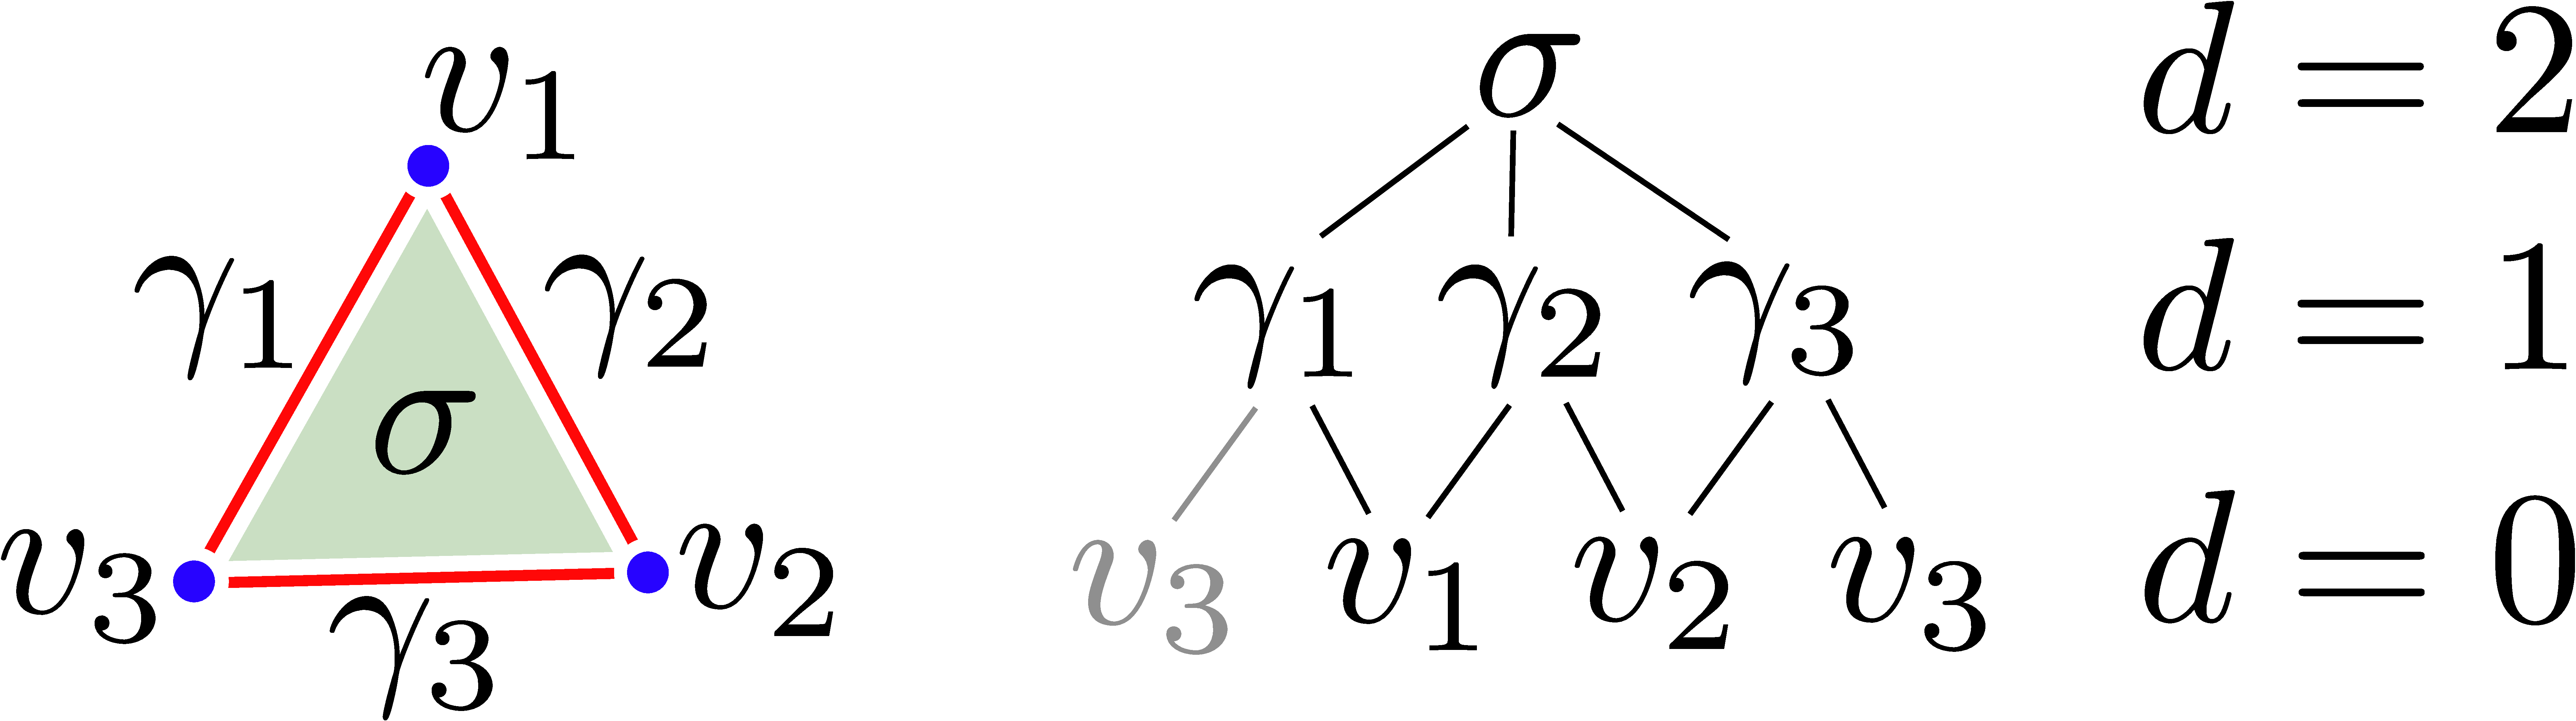
\includegraphics[width = 5.0in]{figures/entity_tree.pdf}
		\caption{A representative entity tree diagram for a $2$-dimensional facet $\sigma$.}
		\label{fig:entity_tree}
	\end{figure}
	
	Additional information may be stored on a given entity (generically denoted as $\omega$), including:
	\begin{itemize}
		\item A reference coordinate $\mathbf{X}_\omega$ which lies on the hyperplane that contains $\omega$. (If $\omega$ is a vertex, $\mathbf{X}_\omega$ is uniquely defined.)
		\item The monomial moments $\int_{\omega} \mathbf{X}^\alpha \, d \omega$ for all $|\alpha| \leq k$, where $k$ is prespecified (or the shifted monomial moments $\int_{\omega} (\mathbf{X}-\mathbf{X}_{\omega})^\alpha \, d \omega$).
		\item Information (pointers or IDs) regarding the $(d+1)$-dimensional parents of $\omega$.
	\end{itemize}
	
	The advantage of defining entities in this fashion is that it affords added flexibility in evaluating monomial moments on arbitrary polytopes, and in solving (\ref{eq:dg_poisson}) on domains with arbitrary dimensionality.
	
\subsection*{Sub-Elements}

	Herein, a \textit{sub-element} is defined as a generic data structure which contains the partitioned geometry for a given polyhedral element, polygonal face, linear edge, or node. A given $d-$dimensional sub-element (henceforth generically denoted as $\Omega$) consists of a collection $d$-dimensional entities, and all $(d-1)-$dimensional sub-elements constituting the boundary of $\Omega$. A sub-element of dimension $0$ (a node) refers to a single vertex, and possesses no bounding sub-elements.
	
	
	
\section{Hierarchial Construction of Appoximants}

\section{Issues of Numerical Conditioning}
\subsection{PEM Linear System Conditioning}
\subsection{The Effect of Element Scaling}
\subsection{On the Choice of an Appropriate PEM Basis}
